\documentclass[lang=cn,10pt,green]{elegantbook}
\usepackage{subcaption} % 引入 subfigure 宏包
\title{2025年中级宏观经济学笔记}
\subtitle{授课: 余昌华老师}

\author{徐靖}
\institute{PKU}
\date{Febuary 27, 2025}
\bioinfo{声明}{请勿用于个人学习外其他用途!}

\extrainfo{个人笔记, 如有谬误, 欢迎指正! 联系方式 : 2200012917@stu.pku.edu.cn}

\setcounter{tocdepth}{3}

\logo{logo-blue.png}
\cover{cover.jpg}

% 本文档命令
\usepackage{array}
\newcommand{\ccr}[1]{\makecell{{\color{#1}\rule{1cm}{1cm}}}}

% 修改标题页的橙色带
% \definecolor{customcolor}{RGB}{32,178,170}
% \colorlet{coverlinecolor}{customcolor}

\begin{document}

\maketitle
\frontmatter

\tableofcontents

\mainmatter

\chapter{中国宏观经济概况}

这节没什么知识, 主要是图表感受一下, 复习可跳过

\begin{figure}[htbp]
    \centering
    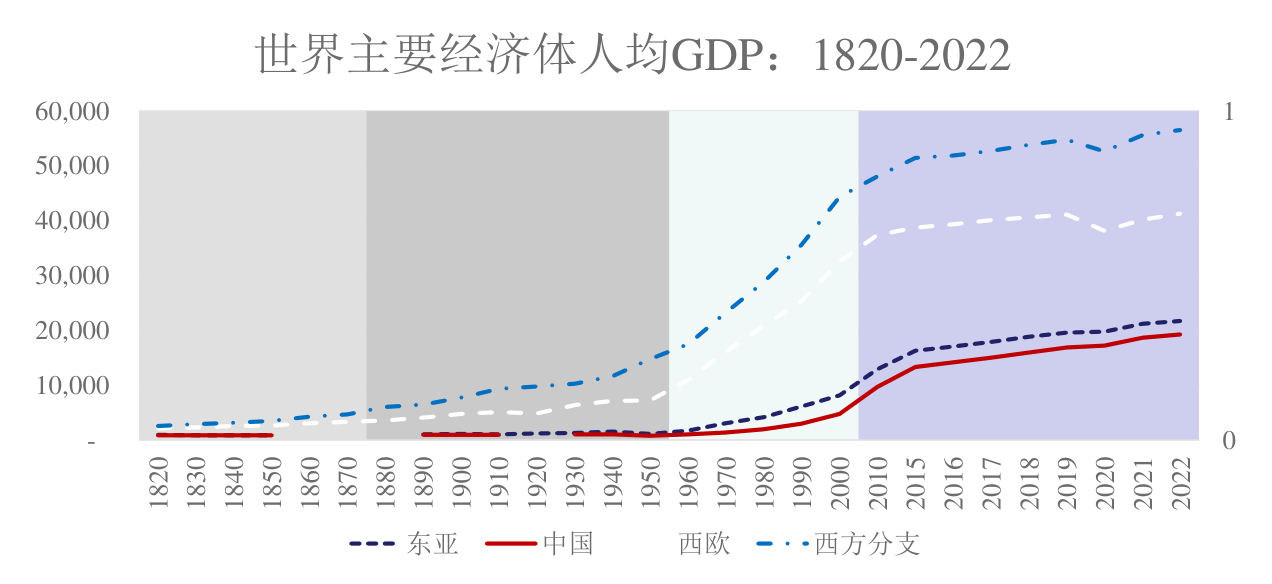
\includegraphics[width=0.8\linewidth]{image/世界主要经济体人均.png}
\end{figure}

\begin{figure}[htbp]
    \centering
    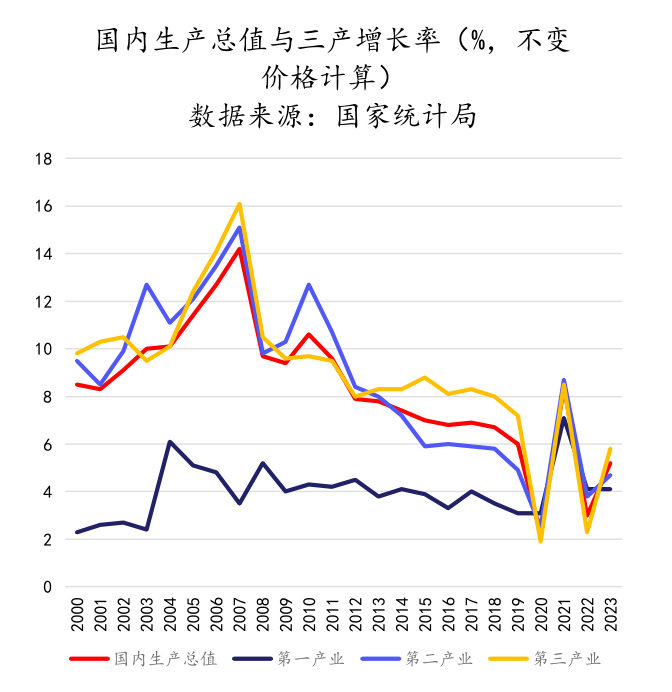
\includegraphics[width=0.5\linewidth]{image/国内生产总值与三产增长率1.png}
\end{figure}

\begin{itemize}
    \item 2000 年以来 GDP 平均增长 8.3\%
    \item 第二产业平均增长 8.7\%
    \item 第三产业平均增长 9\%
\end{itemize}

\newpage

\begin{figure}[htbp] % 使用 [H] 固定位置
  \centering
  \begin{subfigure}[b]{0.9\textwidth}
    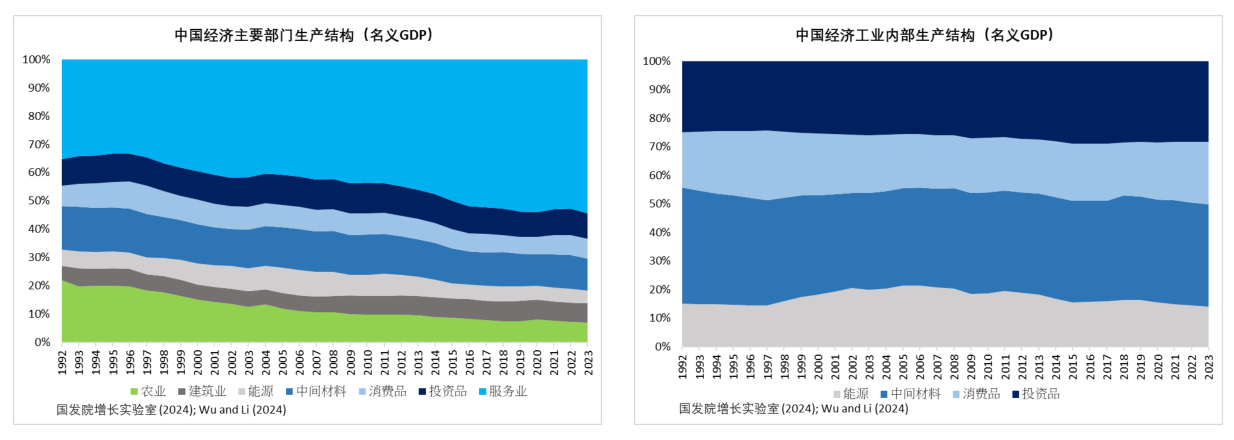
\includegraphics[width=\linewidth]{image/中国经济主要行业构成.png}
    \label{fig:industry}
  \end{subfigure}
\begin{subfigure}[b]{0.9\textwidth}
    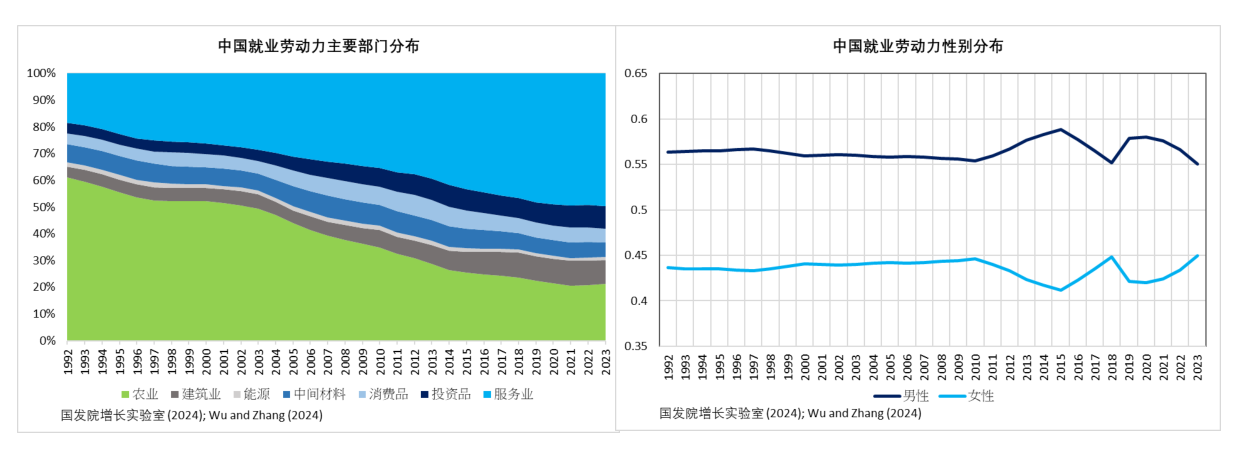
\includegraphics[width=\linewidth]{image/中国就业劳动力行业分布.png}
    \label{fig:labor_industry}
  \end{subfigure}
\begin{subfigure}[b]{0.9\textwidth}
    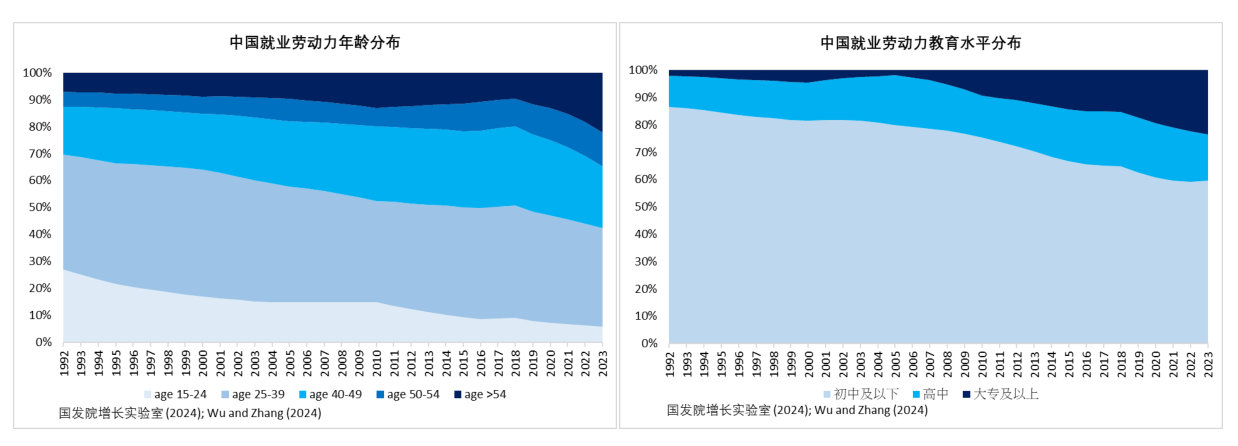
\includegraphics[width=\linewidth]{image/中国就业劳动力年龄与教育.png} % 修正文件名
    \label{fig:labor_age_edu}
  \end{subfigure}
  \label{fig:combined}
\end{figure}
\newpage

\begin{figure}[htbp]
  \centering
  \begin{minipage}[t]{0.35\textwidth}
    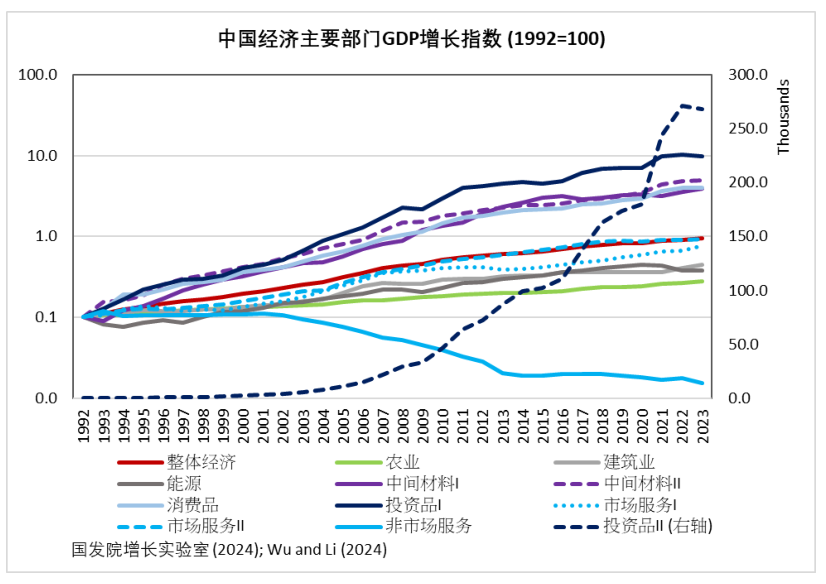
\includegraphics[width=\linewidth]{image/中国经济主要部门增长指数.png}
  \end{minipage}
    \begin{minipage}[t]{0.35\textwidth}
    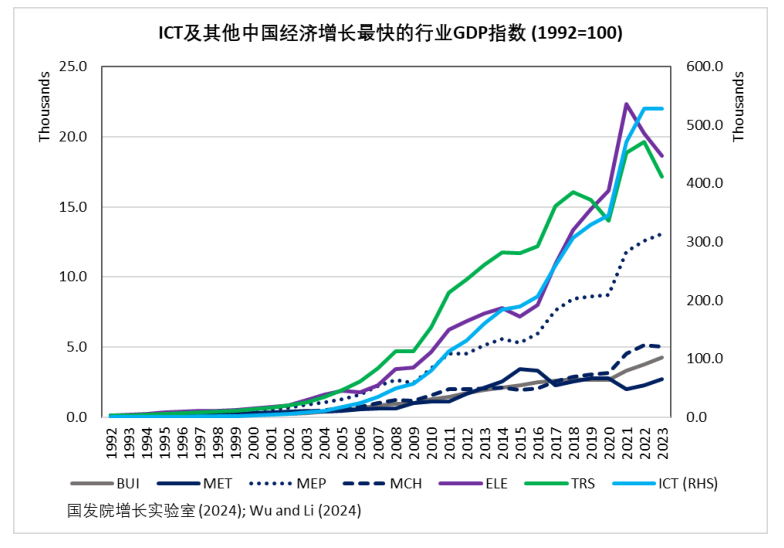
\includegraphics[width=\linewidth]{image/ICT引领行业增长.png}
  \end{minipage}
\end{figure}



\begin{figure}[htbp]
    \centering
    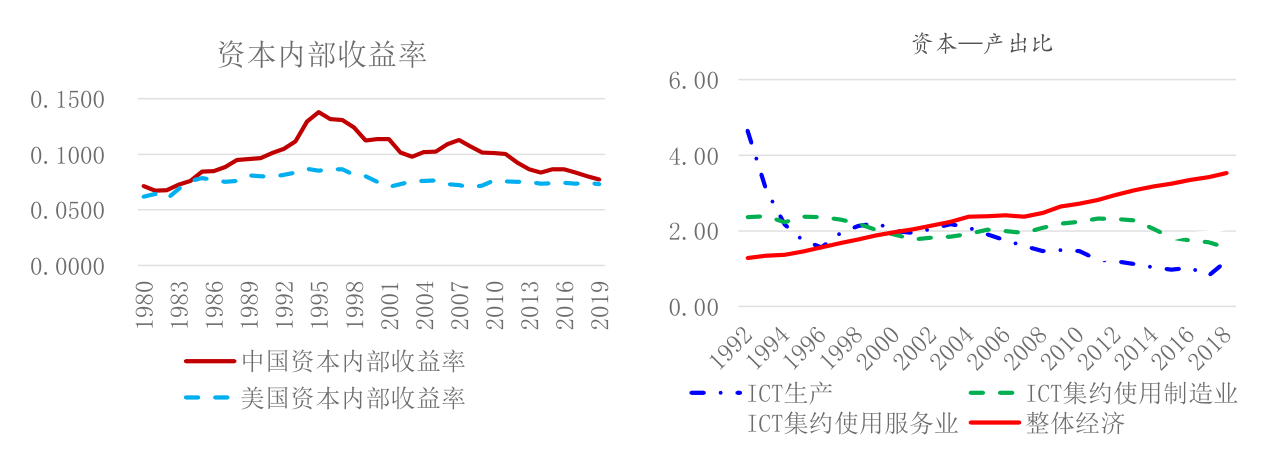
\includegraphics[width=0.75\linewidth]{image/科技赋能助力经济增长.png}
\end{figure}
\begin{figure}[htbp]
    \centering
    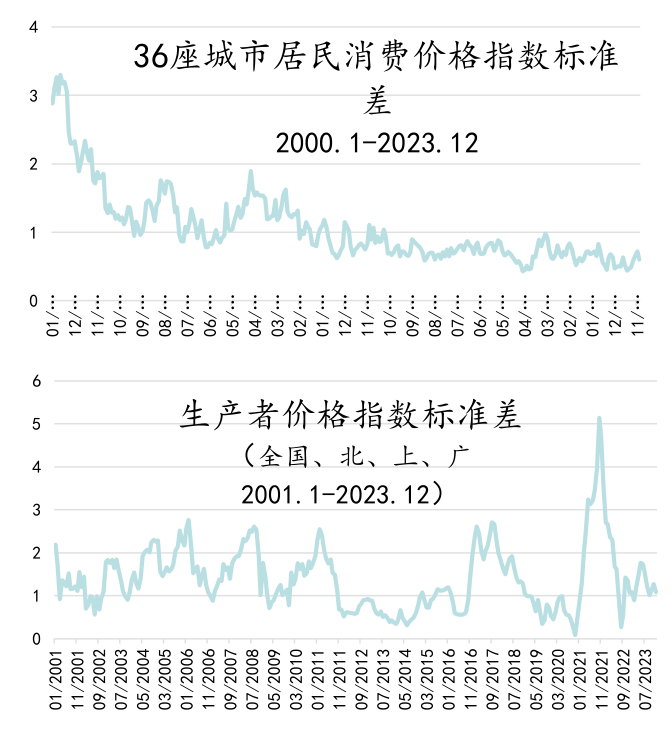
\includegraphics[width=0.4\linewidth]{image/统一市场.png}
\end{figure}

\begin{itemize}
    \item 2000-2022 交通运输、仓储和邮政业增加值年平均增长 7.8\%
    \item 2023年,交通运输、仓储和邮政业固定资产投资增长10.5\%,高于全国固定资产投资7.5\%
    \item 城市间消费价格同步调整增强
    \item 生产者价格同步变动也在增强(疫情期间除外)
\end{itemize}


\chapter{The Science of Macroeconomics}

这节复习也可以跳过, 主打一个散讲. 一些具体展开我认为在相应章节整理更好

\begin{introduction}[Keywords]
\item Macroeconomics 宏观经济学
\item Optimization 最优化
\item Equilibrium 均衡
\item Empiricism 实证主义
\item Endogenous Variables 内生变量
\item Exogenous Variables 外生变量
\item market clearing 市场出清
\end{introduction}

\section{Introduction to economics}

\begin{itemize}
    \item 经济学的范围
    \begin{itemize}
        \item 经济主体与经济资源
        \item 经济学的定义
        \item 实证经济学 (Positive Economics) 与规范经济学 (Normative Economics)
        \item 微观经济学与宏观经济学
    \end{itemize}
    \item 经济学的三大原则
    \begin{itemize}
        \item 第一原则:\textbf{最优化 (Optimization)}
        \item 第二原则:\textbf{均衡 (Equilibrium)}
        \item 第三原则:\textbf{实证 (Empiricism)}
    \end{itemize}
    \item 经济科学:使用数据与模型理解世界
    \begin{itemize}
        \item 科学方法:模型与数据
        \item 因果与相关 (Causation and Correlation)
        \item 经济问题与答案
    \end{itemize}
    \item 最优化:尽力做到最好
    \begin{itemize}
        \item 选择最佳可行方案
    \end{itemize}
    \item 需求、供给与均衡    
    \begin{itemize}
        \item 买家行为
        \item 卖家行为
        \item 供需均衡
    \end{itemize}
\end{itemize}

\section{Important issues in macroeconomics}

\begin{itemize}
    \item (增长): 中国一直是世界上增长最快的经济体之一,截至2018年,实际国内生产总值(GDP)年均增长率为9.5\%。中国是如何实现这一点的?这种高增长是否可持续?为什么?
    \item (老龄化与增长): 人口老龄化对经济的影响——财政可持续性、经济增长、生产率等。
    \item (金融全球化与增长): 金融自由化和全球化的影响。这些是否有助于提高经济增长和生活水平?
    \item (数字经济与增长): 中国如何推动数字经济作为新的增长驱动力?
    \item (危机与财政政策): 在新冠疫情期间,许多国家启动了大规模的财政刺激计划。为什么?效果如何?有哪些后果?财政负担是否可持续?
    \item (金融稳定): 中国最近于2021年初从房地产开发商开始的去杠杆改革。为什么?
    \item (货币政策): 美联储加息对美国经济和中国经济的影响。
    \item (经济增长与经济波动)
\end{itemize}

\section{Macroeconomics requires rigorous analysis and simplification}
\begin{itemize}
    \item 对宏观经济问题进行严谨分析
    \begin{itemize}
        \item 概念
        \item 逻辑关系(经济模型)
        \item 将模型应用于数据(证伪) (falsification)
    \end{itemize}
    \item 个人、企业和政府的总体行为极其复杂
    \begin{itemize}
        \item 简化假设
        \item 关注关键方面和关键渠道
    \end{itemize}
\end{itemize}
\subsection{An example : supply & demand for new cars}
\begin{itemize}
    \item 经济模型是更复杂现实的简化版本,无关的细节被剥离
    \item 展示各种事件如何影响汽车的价格和数量
    \item 假设市场是竞争性的:每个买家和卖家都太小而无法影响市场价格
    \item 变量:
    \begin{itemize}
        \item $Q_d$ = 买家需求的汽车数量
        \item $Q_s$ = 生产者供应的汽车数量
        \item $P$ = 新车的价格
        \item $Y$ = 总收入
        \item $P_s$ = 钢铁的价格(一种投入品)
    \end{itemize}
\end{itemize}

\begin{definition}[General functional notation]
    shows only that the variables are related. $Q^d = D(P,Y)$
\end{definition}
\begin{definition}[specific functional form]
    shows the precise quantitative relationship. $D(P,Y) = 60-10P+2Y$
\end{definition}

\begin{minipage}{0.48\textwidth}
    \begin{itemize}
        \item Demand equation : $Q^d = D(P,Y)$
        \item Supply equation : $Q^S = S(P,P_S)$
        \item An increase in income increases the equilibrium price and quantity.
        \item An increase in $P_S$ increases the market price and reduces the quantity.
    \end{itemize}
\end{minipage}%
\begin{minipage}{0.48\textwidth}
    \centering
    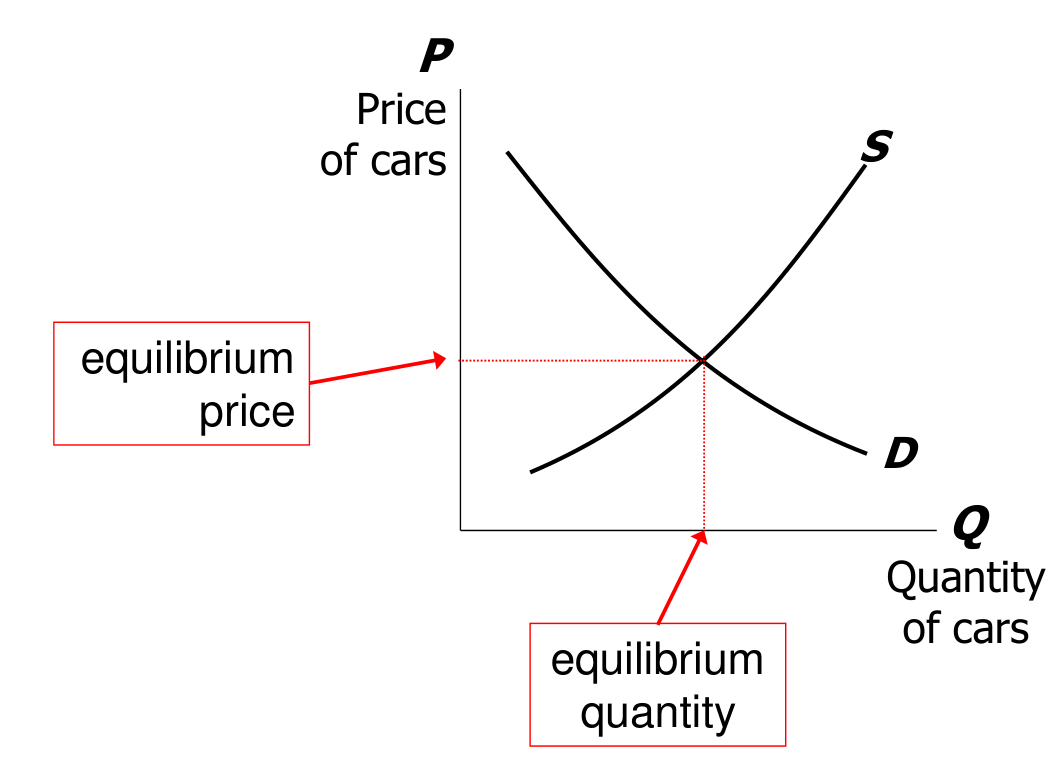
\includegraphics[width=\linewidth]{image/equilibrium of cars market.png}
\end{minipage}

\begin{minipage}{0.48\textwidth}
    \centering
    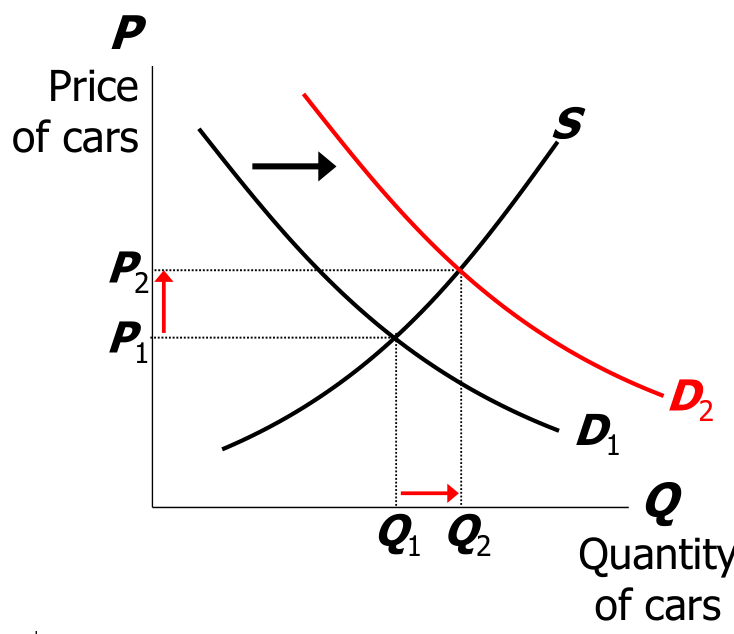
\includegraphics[width=0.8\linewidth]{image/The effects of an increase in income1.png}
\end{minipage}%
\begin{minipage}{0.48\textwidth}
    \centering
    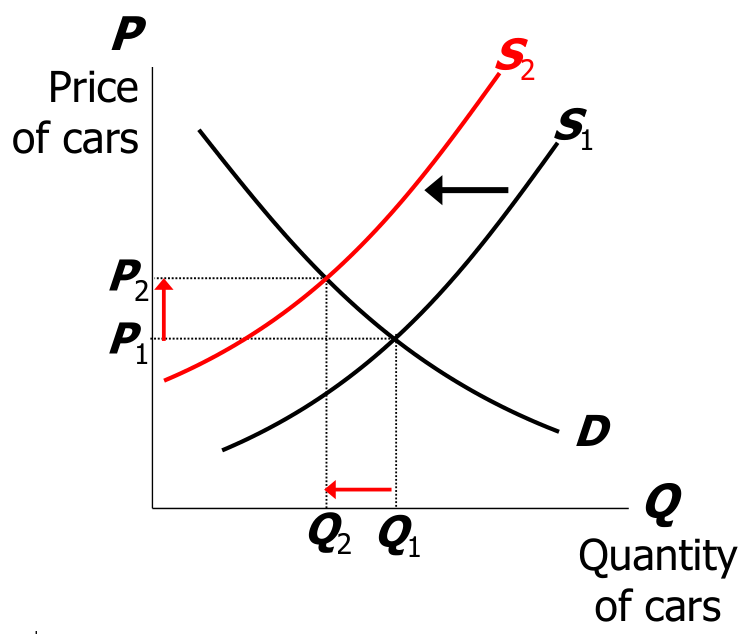
\includegraphics[width=0.8\linewidth]{image/The effects of a steel price increase1.png}
\end{minipage}

\begin{definition}[endogenous variables 内生变量]
    The values of endogenous variables are determined in the model.
\end{definition}
\begin{definition}[exogenous variables 外生变量]
    The values of exogenous variables are determined outside the model. The model takes their values and behavior as given.
\end{definition}

在汽车供需这个模型中,内生变量包括 $P, Q^d, Q^S$,外生变量包括 $Y, P_S$。

\subsection{The use of multiple models}

\begin{itemize}
    \item 没有一个模型能够解决我们所关心的所有问题
    \item 例如,我们关于汽车市场的供需模型
    \begin{itemize}
        \item 可以告诉我们总收入的下降如何影响汽车的价格和数量
        \item 但无法告诉我们总收入为什么会下降
    \end{itemize}
    \item 因此,我们将学习不同的模型来研究不同的问题(例如,失业、通货膨胀、长期增长)
    \item 对于每个新模型,您应注意:
    \begin{itemize}
        \item 其假设
        \item 哪些变量是内生的,哪些是外生的
        \item 它可以帮助我们理解哪些问题,哪些问题无法解释
    \end{itemize}
\end{itemize}

\subsection{Price : flexible vs. sticky}

\begin{definition}[Market clearing 市场出清]
    An assumption that prices are flexible, adjust to equate supply and demand
\end{definition}
\begin{itemize}
    \item 在短期内,许多价格具有粘性 (sticky) ———— 对供应或需求变化的反应迟缓 (sluggishly)。例如
    \begin{itemize}
        \item 许多劳动合同将名义工资 (nominal wage) 固定一年或更长的时间。
        \item 许多杂志出版商每 3 至 4 年才变动一次价格。
    \end{itemize}
    \item 经济行为在一定程度上取决于价格是粘性的还是弹性的: 
    \begin{itemize}
        \item 如果价格具有粘性(短期),需求可能不等于供给,这解释了:
        \begin{itemize}
            \item 失业(劳动力供给过剩)
            \item 为什么企业不能总是卖出其生产的所有产品?
        \end{itemize}
    \end{itemize}
    \item 如果价格具有弹性(长期),市场就会出清,经济行为就会截然不同。
\end{itemize}

\end{document}
